\svnInfo $Id: einleitung.tex 72 2008-04-06 17:42:54Z axel $
\chapter{Einleitung}

\section{Motivation}
Der Großteil der interaktiven 3D-Anwendungen, die heutzutage auf dem Markt sind, werden mittels des Rasterisierungsverfahrens und der dafür angepassten Hardware umgesetzt. Dabei werden die einzelnen Dreiecke, aus denen die virtuelle Szene zusammengesetzt ist, unabhängig voneinander behandelt. Dadurch wird eine effiziente, parallele Implementierung des Algorithmus in speziell dafür gestalteter Hardware, die in nahezu allen Grafikkarten eingebaut ist, möglich.
Die wachsenden Anforderungen an die Qualität der dargestellten Bilder erhöht jedoch zunehmend die Komplexität der Programme, die diese Technologie nuzten. Gerade bei Objekten deren Erscheinung von anderen Objekten abhängt (zum Beispiel bei Schattenwurf) wird die Simulation nicht vom Rasterisierungsverfahren abgedeckt.
Komplexe Beleuchtungsszenarien werden deshalb oft in Software vorbereitet und mit in der Szenenbeschreibung abgespeichert.
Das Raytracingverfahren bildet mit seinem physikalisch motivierten Ansatz eine alternative Vorgehensweise. Der Fluss des Lichts von den Lichtquellen zum Auge des Betrachters wird durch die Verfolgung von virtuellen Lichtstrahlen simuliert. Dieser allgemeine Ansatz ermöglicht die Darstellung vieler realistische Phänomene ohne sich dem Programmiermodell einer bestimmten Hardwarestruktur anpassen zu müssen.
Durch seinen hohen Rechenaufwand wurde das Verfahren bis vor wenigen Jahren für Echtzeitdarstellungen nicht in Betracht gezogen. Die steigende Rechenleistung ermöglichte in den letzten Jahren erfolgreiche erste Implementierungen mit interaktiven Frameraten auf gewöhnlichen Arbeitsplatzrechnern.


\section{Struktur der Arbeit}

Die Arbeit gibt eine Einführung in die Themengebiete mit denen sich ein Softwareentwickler auseinandersetzten muss, um eine effiziente Implementierung eine Raytracers zu entwickeln. Zu diesem Zweck werden in Kapitel \ref{chap:rt} zunächst die grundlegende Vorgehensweise des Raytracingverfahrens und die dabei zu lösenden Probleme aufgezeigt.
Kapitel \ref{sec:introstructs} zeigt mittels welcher Algorithmen das Kernproblem, die Bestimmung eines Schnittpunktes von einem Strahl und der Szenengeometrie, effizient gelöst werden kann.
Die Implementierung dieser Algorithmen auf einem Computer bringt gewisse Implikationen mit sich. Eine naive Umsetzung kann die Effizenz der angwendeten Verfahren um Größenordnungen herabsetzen. Deswegen werden in Kapitel \ref{chap:Hardware} verschiedene Eigenschaften aktueller Computer, und Richtlinen zur Entwicklung effizienter Anwendungen auf solchen, vorgestellt.
Im letzten Kapitel \ref{chap:fazit} wird auf die praktische Entwicklung einer Raytracinganwendung eingegangen und ein Überblick über die im Zusammenhang mit dieser Arbeit entwickelte Software gegeben.
Am Rand mancher Seiten befinden sich Anmerkungen mit den Symbolen 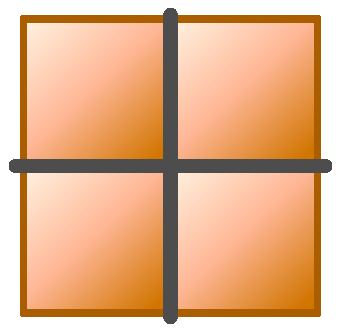
\includegraphics[width=7pt]{images/package.pdf} 
\includegraphics[width=6pt]{images/class.pdf}\includegraphics[width=6pt]{images/method.pdf}. Diese verweisen auf die Stellen im Quellcode an denen ein zuvor beschriebener Algorithmus zu finden ist. Das Beispiel auf dieser Seite verweist auf die Methode \verb|helloWorld| der Klasse \verb|MyClass| im Verzeichnis \verb|examples|.\srcref{examples}{MyClass}{helloWorld}
